\appendix
\section{Details}
We collected the POI categories in all of the five trajectory datasets
and their names with the corresponding icons are shown in figure \ref{fig:poicats}.

Three POI features used to rank POIs, namely, the popularity, 
the total number of visits and the visit duration, in all five datasets are shown in 
figure \ref{fig:popularity}, figure \ref{fig:nvisit} and figure \ref{fig:duration} respectively.

Figure \ref{fig:transmat} shows the heat map of the transition matrices for $5$ individual POI features
in Melbourne dataset.


\begin{figure}
\centering
%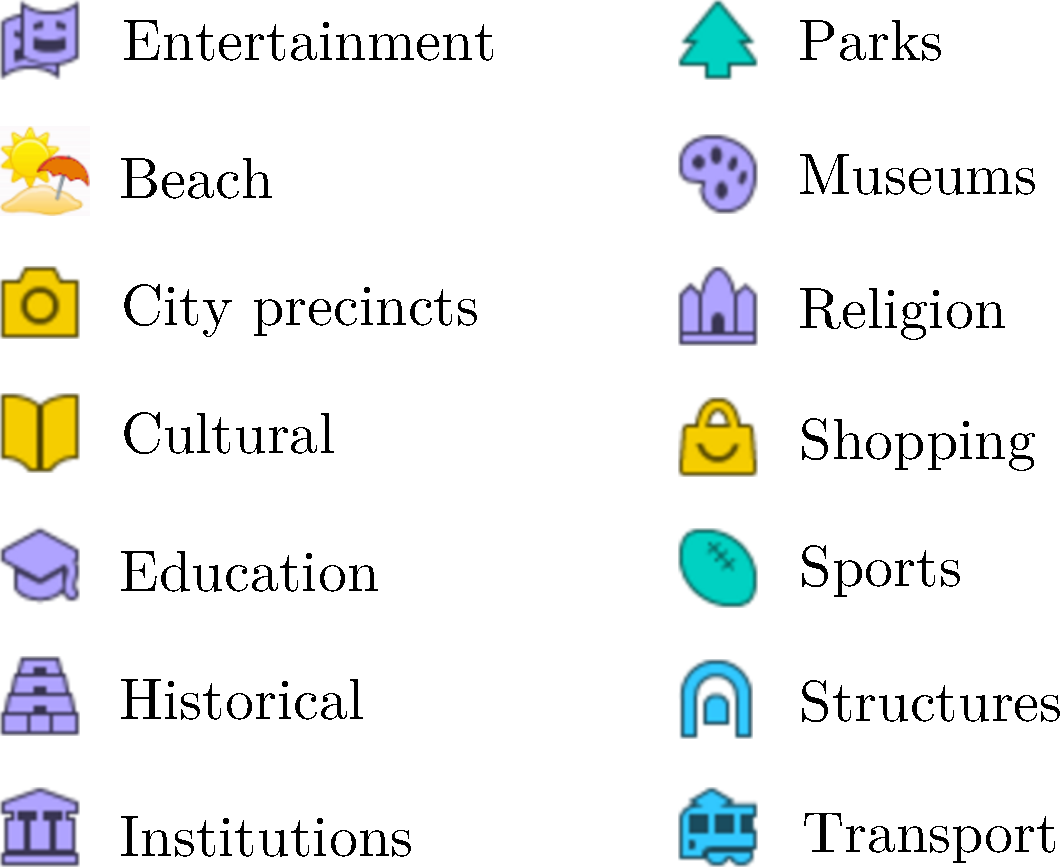
\includegraphics[width=\columnwidth]{fig/poi_cats.pdf}
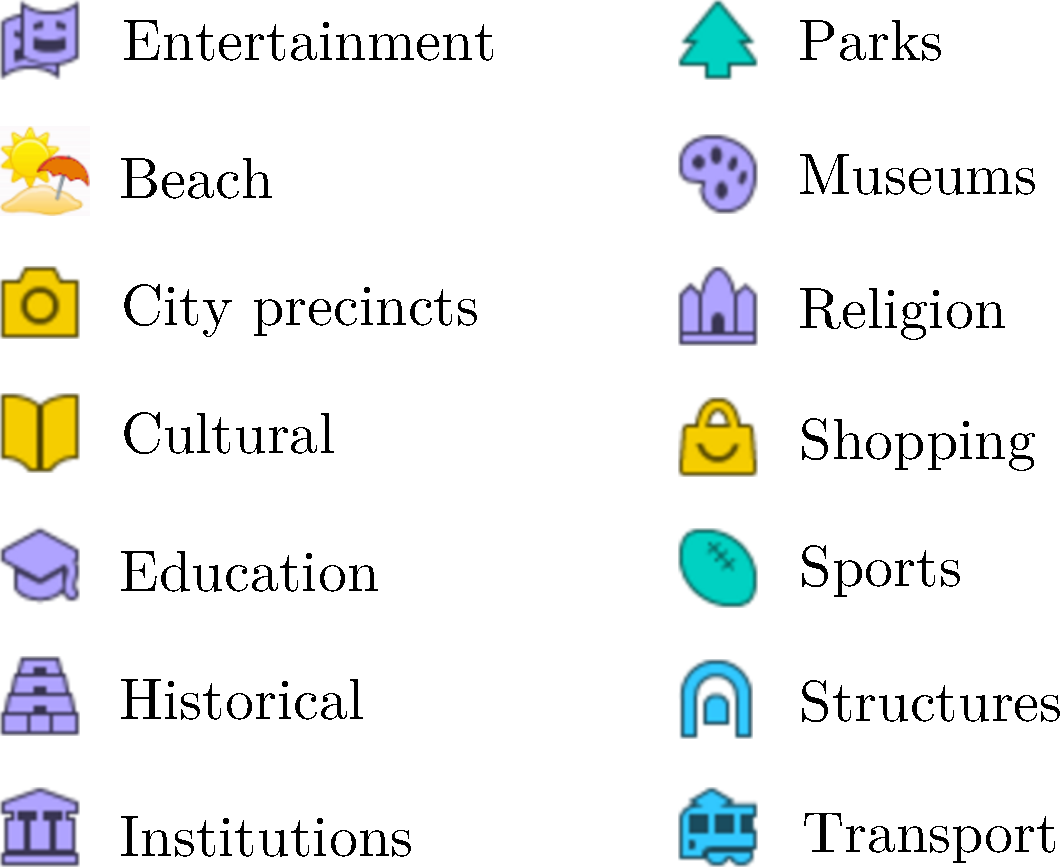
\includegraphics[scale=.32]{fig/poi_cats.pdf}
\caption{POI categories}
\label{fig:poicats}
\end{figure}

\begin{figure*}
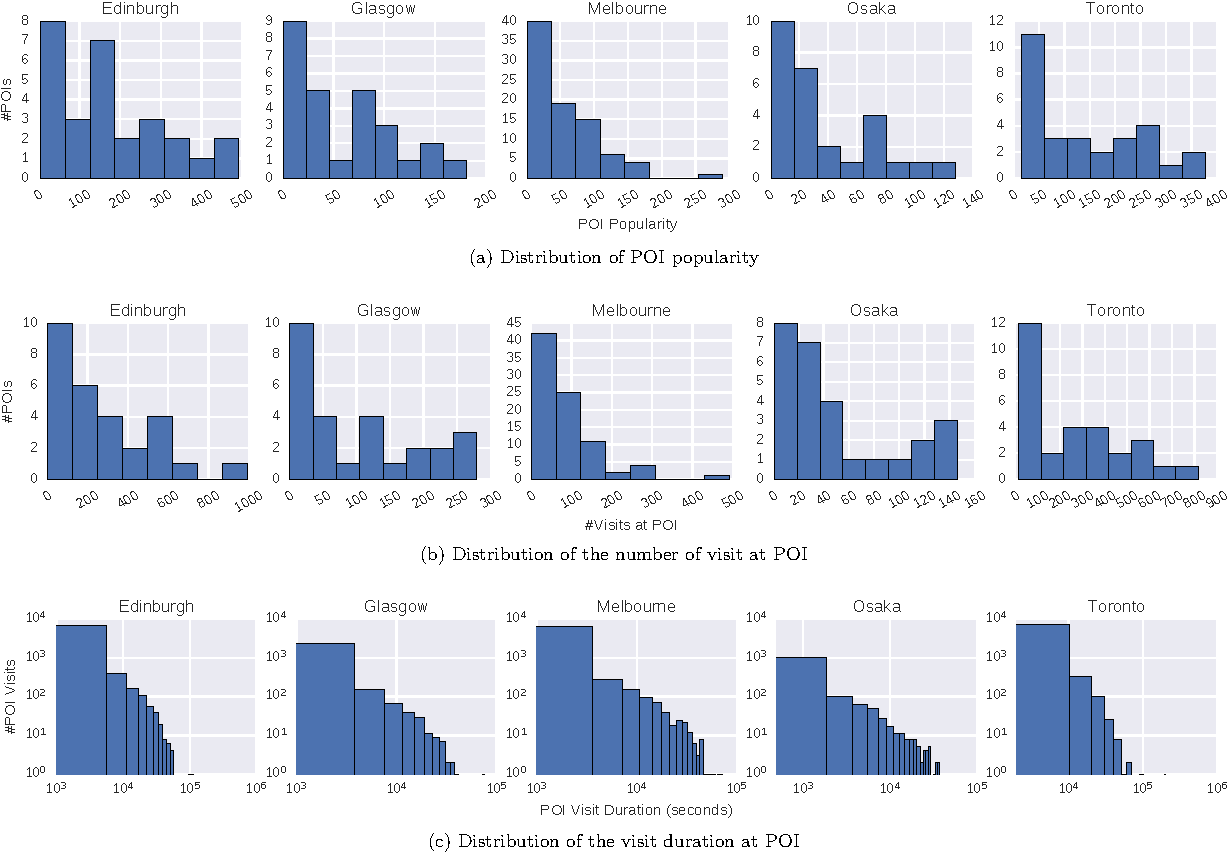
\includegraphics[width=\textwidth]{fig/feature_distro.pdf}
\caption{Distribution of POI popularity, the number of visit and visit duration}
\label{fig:distro}
\end{figure*}

An example of trajectory with four POIs from Toronto dataset was shown in figure \ref{fig:traj},
%TODO: explain what is a POI/photo in the figure
where the four colored marker icons represent the four POIs,
and the colored round icons represent a sample of photos assign to these POIs.


\begin{figure}
\centering
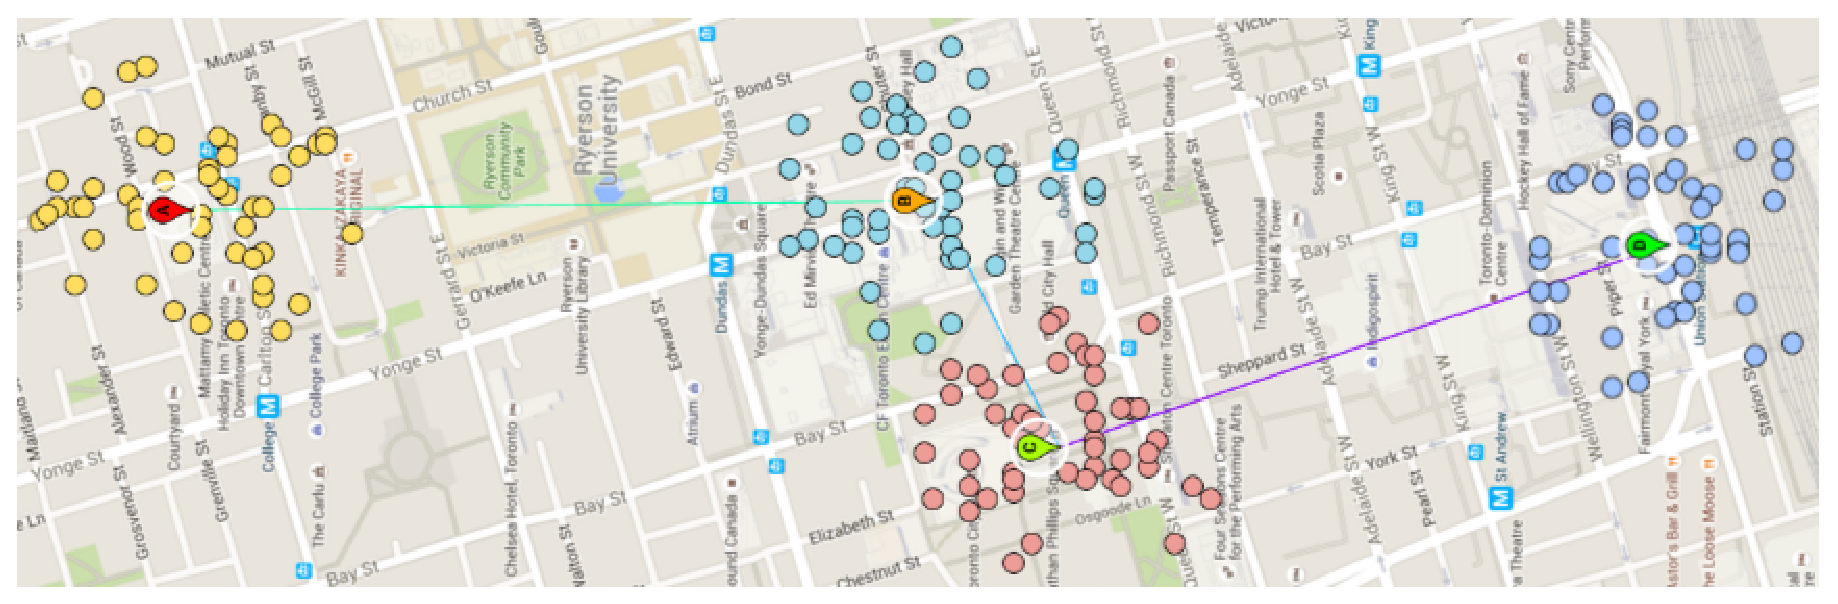
\epsfig{file=fig/traj_eg.eps, width=3.5in}
\caption{An example of trajectory with four POIs}
\label{fig:traj}
\end{figure}



\section{POIs with same features}


By computing the Kronecker product of transition matrices of all the POI features,
we get an unnormalised transition matrix of POI features.
However, to obtain the transition probabilities between each POI pair $(p_i, p_j)$,
there are two cases needs to be dealt with properly:
\begin{enumerate}
\item POI features which represent POIs that do not exist in $\mathcal{P}$,
\item POI features that corresponds to more than one POIs in $\mathcal{P}$.
\end{enumerate}

% deal with feature vector without corresponding POI or with more than one POIs.
For the first case,
the corresponding rows and columns in the result matrix of Kronecker product are simply removed.

The second case was a bit subtle.
Let POIs with exactly the same features be a POI group,
the transition probabilities associated with POIs in the same group are computed as follows:
\begin{itemize}
\item The incoming (unnormalised) transition probability of the group was divided uniformly among POIs
      in the same group, which is equivalent to choose a POI in the group uniformly at random;
\item The outgoing (unnormalised) transition probability of each POI should be the same as the
      outgoing transition probability of the POI group, as one had already been in the POI group in this case;
\item The self-loop of the POI group represents the transitions between POIs in the same group,
      suppose the (unnormalised) transition probability from a POI group to itself is $P_o$,
      and the number of POIs in the group is $N_o$,
      the transition probability from $p_i$ to $p_j$ in the same group is
      \begin{displaymath}
          P(p_j | p_i) =
          \begin{cases}
              \hfill 0, \hfill & i = j \\
              \hfill \frac{P_o}{N_o - 1}, \hfill & i \ne j \\
          \end{cases}
      \end{displaymath}
\end{itemize}
Finally, the unnormalised outgoing transition probabilities of each POI were normalized to form
a valid probability distribution
\footnote{Note that dealing with the second case before or after the normalization leads to
the same transition probabilities, which can be easily proved. \cheng{Show proof}}.


\section{Avoid Peeking}
When working with machine learning algorithms, to make sure the reported performance is a good approximation
of the generalization performance, it is critical to prevent information in test set from leaking into
training set.
Many algorithms in the above comparison utilizing both learning to rank and factorized transition matrix,
e.g., \textsc{Rank+Markov}, \textsc{Rank+MarkovPath} and \textsc{StructuredSVM},
both of them need to be trained or parameters be estimated before being utilized in other algorithms.
Features such as popularity of a POI, the number of visits of a POI and the average visit duration at a POI are
determined by not only the POI itself but also trajectories in training set, let's call them aggregated features as they are
computed by aggregating a set of trajectories.
To make sure the prediction performance is reliable, it is very important to exclude trajectories in test set
when computing aggregated features.
Unfortunately, it is quite easy, especially when utilizing multiple levels of machine learning models,
to use all data, including those in test set, to compute aggregated features and many researchers and
practitioners did not realize some bits of information in test set were leaked into training set via these aggregated features.

%One may argue that many of these features will not change much when computed with or without data in test set,
%but in certain areas, such as aerodynamics, some decisions are very sensitive to the quantity of certain features.
%Nevertheless, the exact impact still needs further investigation.

\section{Implementation details}
libsvmtools, PyStruct, Gurobi, etc.

There are about $12$\% of trajectories in Melbourne dataset that were failed to be evaluated
using \textsc{PersTour} due to the timeout of integer programming solver, the timeout is $2$ hours.
